\chapter{MIP Timing Detector}

In the coming years the LHC will be working toward upgrades that will lead a substantial increase in luminosity.  The timeline for future operations of the LHC is shown in Figure \ref{fig:lhctimeline}.  In 2019 the LHC entered a two-year shutdown, Long Shutdown 2 (LS2).  Upgrades of the LHC injector complex to increase the beam brightness will take place during this shutdown.  After LS2 the LHC will enter Run 3 which will run for three years at 13-14 TeV.  At the completion of Run 3 the LHC will enter Long Shutdown 3 (LS3) which will last approximately 2.5 years.  During LS3 the optics in the interaction region will be upgraded to produce smaller beams at the interaction point.  The completion of this upgrade will usher in the High Luminosity (HL-LHC) era or Phase 2 of LHC operations, during which the combination of brighter beams and a new focusing scheme at the IP allows for a potential luminosity of 2x10$^{35}$ cm$^{-2}$s$^{-1}$ at the beginning of each fill \cite{Apollinari:2017cqg}.  

\begin{figure}[h]
	\centering
	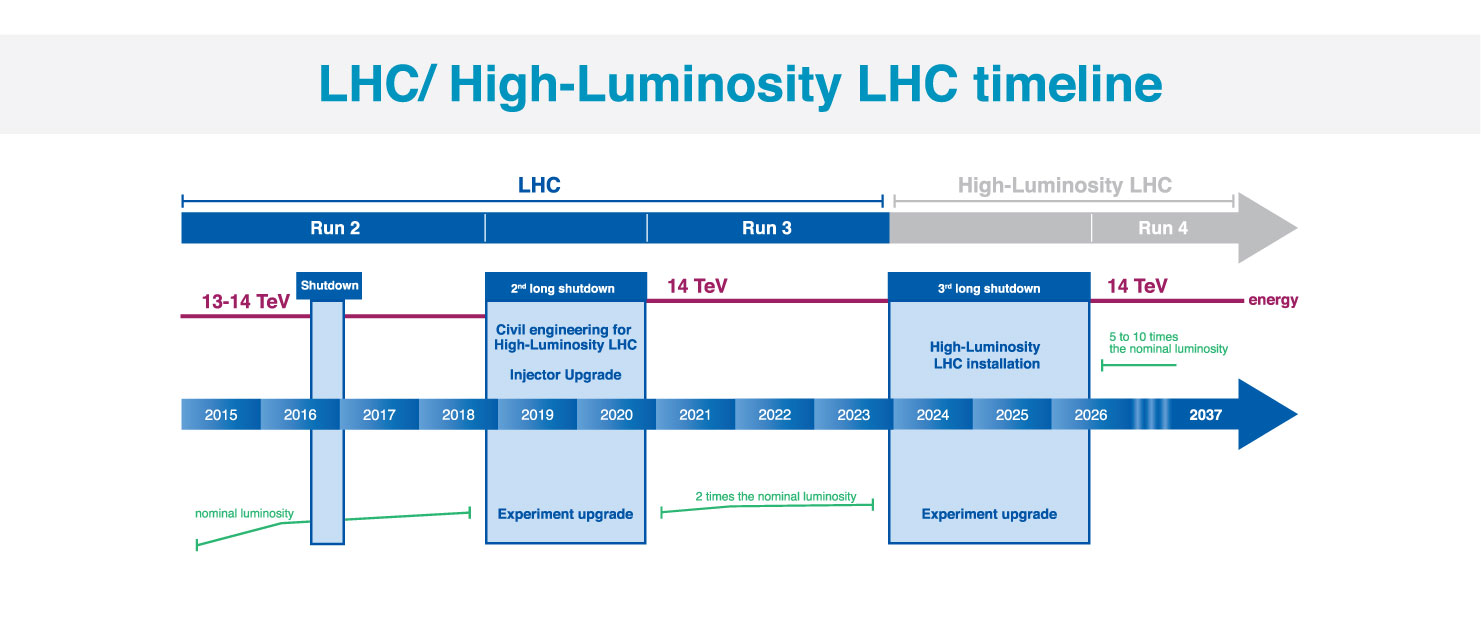
\includegraphics[width=1.0\linewidth]{Figures/LHCTimeline}
	\caption[Timeline for LHC]{Timeline for LHC \cite{DeMelis:2063307}}
	\label{fig:lhctimeline}
\end{figure}

The increased luminosity results in more interactions per bunch crossing or pileup.  In order to limit the amount of pileup the experiments must disentangle to more manageable levels, the nominal scenario would be operating at a stable luminosity of $5.0\times10^{34}$ cm$^{-2}$ s$^{-1}$.  This would limit the pileup to an average of 140.  The ultimate scenario for operations would be running at $7.5\times10^{34}$ cm$^{-2}$ s$^{-1}$ which brings the average pileup up to 200.  The CMS detector in its current state is not capable of dealing with $\approx$140-200 pileup so significant upgrades are necessary in order to maintain the performance in efficiency, resolution, and background rejection that exist at the current level of pileup.  One such upgrade is the addition of a minimum ionizing particle (MIP) Timing Detector (MTD).


